\chapter{Presentation}
\label{chap:intro}

\section{Introduction}

The aim of this chapter is to contextualize our work.
We will start by introducing the hosting institution for the graduation project.
Then, we will present the project, its motivations, and its objectives.
And finally, we will discuss the development process used throughout the making of this project.

% The world has been seeing a continuous shift to remote work since the
% internet boom in the early 2000s. The recent global pandemic instantly
% boosted the number of remote workers to unprecedented levels. On top of
% that, businesses have been gradually moving away from brick-and-mortar
% stores to online software-managed ones. Furthermore, client-side web
% apps and no-code web apps and websites have experienced a surge in the
% number of users. These factors uncovered a gap in the niche of
% easy-to-use collaborative data and content management software.

\section{Host}

This project is done as part of the final graduation project with the goal of obtaining the License Degree in Computer Science within the Higher School of Sciences and Technology of Hammam Sousse.

\section{Project presentation}

Our project's main idea and design choices stem from the problems we faced while trying to accomplish certain tasks using other tools.
% A robust implementation of our project requires deep research of multiple aspects that will guide our design and implementation decisions.

\subsection{Problematics}

The continous shift to \acrfull{saas}, coupled with the rise of remote work, uncovered a gap in the field of data and content management software. The gap is further exacerbated due to the accelarting adoption of web applications, which are mostly client-side applications without any server requirements. Nowadays, businesses are looking for easy and collaborative ways to allow stakeholders to manage data and content, and to connect the data to their different applications. The solution must respond to the needs of businesses from different backgrounds, with varying budgets, and minimal technical knowledge. The solution must also be easily intergratable with other tools that these businesses might rely on. Furthermore, the solution must support recent technilogical advancements in the web, such as real-time collbaoration and real-time queries. To ensure these requirements, we need to answer the following questions:

\begin{itemize}
	\item How to support real-time collaboration?
	\item What level of collaboration is required for optimal productivity?
	\item How should we organize and share data between multiple users?
	\item What interface structure ensures the most accesible software?
	\item What data types should we support?
	\item How important is speed?
	\item How can we ensure a fast user experience?
	\item What are the bottlenecks of the existing solutions and how can we solve them?
	\item How can we ensure a fast and easy on-boarding?
\end{itemize}

\section{Preliminary study}

Before starting the development process of our projects, it is of utmost importance to research the existing solutions in the field of data and content management that our potential users are currently relying on.
It is necessary to understand what problems users are facing while using these solutions and what kind of tricks and shortcuts do they have to depend on to achieve their desired outcome. We should also focus on the points that users admire about their current choices, as these are the features keeping them from looking for another solution in the meantime.

With this goal in mind, we went on to research multiple applications and software systems with varying degrees of features and requirements.
While some might require deep technical knowledge of databases, servers, and programming, others are more straightforward and require little to no technical knowledge.
However, while some applications may require no programming skills, they still require some time for on-boarding and getting familiar with the software.
This can be a significant roadblock for many entreprises that are already stuck with some other software system.

From this wide pool of data and content management software, we selected the most used and loved ones and put them to comparison. In particular, we chose to focus on PostgREST, Notion, Airtable, Contentful, Sanity, Webflow CMS, and Firebase.

\subsection{Existing solutions}

We will start by presenting the selected solutions.

\subsubsection{PostgREST}

\begin{figure}[h]
	\centering
	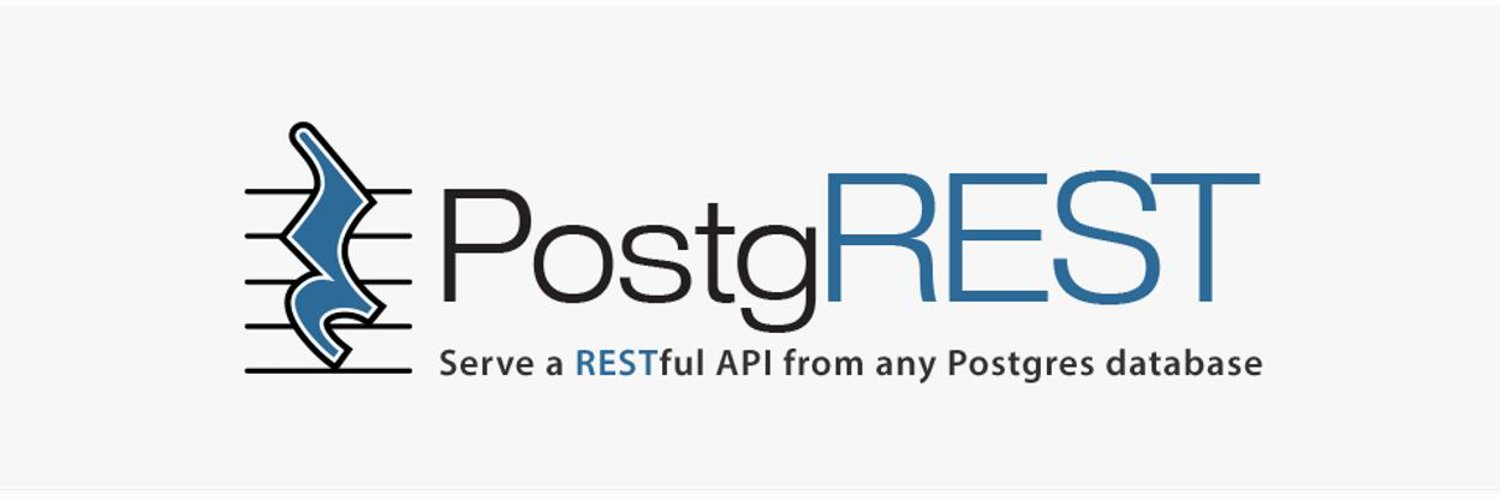
\includegraphics[width=\linewidth]{postgrest-logo.png}
	\caption{PostgREST logo}
\end{figure}

PostgREST is an automatic API generator for Postgres databases.


\subsubsection{Firebase}

\begin{figure}[h]
	\centering
	
\includegraphics[width=\linewidth]{firebase-logo.png}
	\caption{Firebase logo}
\end{figure}

Firebase is a platform developed by Google for creating mobile and web
applications. It was initially released in 2012. It offers, among its
products, a real-time database. In which, data is stored in JSON format
and synced between all the connected clients. The database was not
developed with non-technical users in mind, however, its real-time
capabilities offer an example of what's desired in real-time database
software. Firebase Realtime Database has been successfully used to
develop highly demanding mobile applications.

\subsubsection{Airtable}

\begin{figure}[h]
	\centering
	
\includegraphics[width=\linewidth]{airtable-logo.png}
	\caption{Airtable logo}
\end{figure}

Airtable is a visual database app inspired by the ease of spreadsheets
and the wide adoption of software like Microsoft Excel. The company
behind the app was founded in 2012.

Airtable comes with team collaboration out of the box. It also
automatically generates a REST API from each database.

Pricing is done per team member. There are several limits to the size of
storage and uploads.

\subsubsection{Contentful}

\begin{figure}[h]
	\centering
	
\includegraphics[width=\linewidth]{contentful-logo.png}
	\caption{Contentful logo}
\end{figure}

Contentful is a headless\footnote{Content is decoupled from the main
	application. It's made accessible through a set of APIs.} CMS (Content
Management Software). It offers a flexible CMS editor and a configurable
API. It also comes with multiple SDKs (Software Development Kits) in
multiple programming languages to make its integration easier.

Pricing is offered per package, with the lowest premium package starting
at US\$489 per month.

\subsubsection{Sanity}

\begin{figure}[h]
	\centering
	
\includegraphics[width=\linewidth]{sanity-logo.png}
	\caption{Sanity logo}
\end{figure}

Sanity.io is another headless CMS. It competes directly with Contentful,
offers an even more configurable editor, and its pricing starts at
US\$199 per month. It comes with real-time collaboration, a feature that
Contentful lacks.

\subsubsection{Webflow CMS}

\begin{figure}[h]
	\centering
	
\includegraphics[width=\linewidth]{webflow-logo.png}
	\caption{Webflow logo}
\end{figure}

Webflow is a website builder. It bundles a CMS and an e-commerce
management system along with its visual website builder. The CMS is not
usable outside of Webflow websites, however, it comes with an intuitive
user interface.

\subsubsection{Notion}

\begin{figure}[h]
	\centering
	
\includegraphics[width=0.5\linewidth]{notion-logo-2.png}
	\caption{Notion logo}
\end{figure}

Notion is a new contender in the space of content management. It
presents itself as a collaborative workspace for teams. Its use cases
vary from product management and team documentation to note-taking and
personal organization. The initial version of Notion was released in
2016. The second version, which received a lot of praise and media
coverage, was released two years later in 2018. However, the largest
surge in signups happened during the pandemic, with 40\% of signups
occurring from December 2020 to January.

Notion.so is built on the concept of blocks: A block is any single piece
of content you add to your page, like a to-do item, an image, a code
block, an embedded file, etc. \footnote{citation needed, see Notion FAQ}
This makes it easy to build complex pages and move content around.

Notion is also built as a collaborative web app---eliminating the need
for saving and figuring out how to share one's documents as is the case
in other apps.

Pricing is done per workspace member with unlimited storage starting
from the free plan.

\subsection{Critique}

Multiple solutions are trying to focus on various use cases, however,
all of them suffer from noticeable performance issues, a bad UX (User
Experience), and inadequate pricing for small and medium-sized
businesses.

Notion is known for its slow performance and long loading times. Pages
take on average between six and 12 seconds to load. \footnote{citation
	needed} It also doesn't have an API, although one is being developed
at the time of writing. Furthermore, Notion is less structured than
products like Airtable or Firebase.

Airtable is notable for its complexity, even for experienced users. It
also suffers from some performance issues when loading large documents.
Furthermore, it doesn't have the same rich text capabilities as Notion.
Finally, it lacks a real-time API and it's relatively expensive.

\subsection{Proposed solution}

Merebase is a collaborative visual database that can be used for data
and content management. It's built with real-time collaboration,
performance, and intuitiveness in mind. Thanks to years of innovation in
the field of browser apps and high-performance real-time servers, it
should be able to load instantaneously, while offering a smooth user
experience with no glitching or slowdowns when loading large documents,
and with the ability to effortlessly collaborate with other users.

\section{Conclusion}

The recent changes in workplaces and software development require robust
collaborative and intuitive visual database systems, which we currently
lack. Merebase is a proposed solution for these problems, built on top
of cutting-edge technologies to offer the best user experience possible.